\capitulo{3}{Conceptos teóricos}
\label{ConceptosTeoricos}

El procesamiento de imágenes toma un papel muy importante en este proyecto. El objetivo es la detección de perikymata y para ello en esta sección se abordarán conceptos teóricos importantes sobre el preprocesado que se ha llevado a cabo y el marcado y detección de bordes.

El preprocesado está formado por la \textit{ecualización adaptativa del histograma}, la \textit{reducción de ruido} y la \textit{aplicación de filtros} de detección de bordes. El marcado de bordes comprende la \textit{binarización} de la imagen y la \textit{esqueletonización} y para finalizar la detección de bordes se lleva a cabo mediante la aplicación de la \textit{transformada de Hough} y el uso del espacio de color \textit{HSV}.

\section{Ecualización adaptativa del histograma}
\label{EcualizacionAdaptativa}
La operación de ecualización adaptativa del histograma\footnote{Se conoce también como \textit{AHE} (\textit{Adaptative Histogram Equalization}).}  se realiza sobre una imagen para conseguir un mayor contraste. Una modificación de esta operación es la que lleva a cabo el algoritmo \textit{CLAHE} \cite{wiki:CLAHE} (\textit{Contrast Limited Adaptive Histogram Equalization}) el cual toma cada píxel de la imagen y su vecindario sobre los que extrae el histograma y realiza la ecualización, de este modo se consigue una ecualización local en vez de una global y con ello un marcado de bordes más adecuado para el tema que nos ocupa como vemos en la figura \ref{LennaEqua}.

\begin{figure}[H]
\centering
\subfloat[Imagen original \cite{wiki:Lenna}]{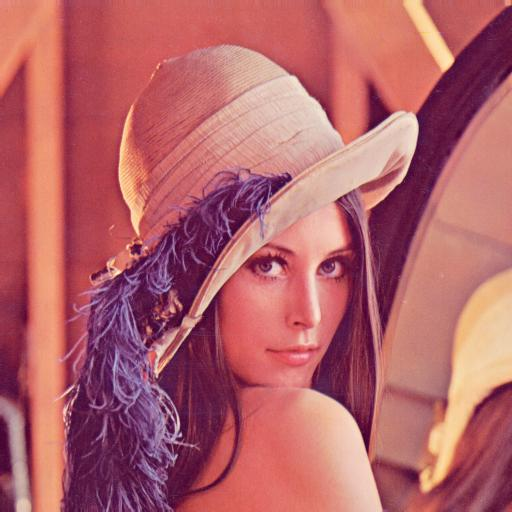
\includegraphics[width = 2.15in]{img/ConceptosTeoricos/LennaOriginal}}
\subfloat[Imagen ecualizada]{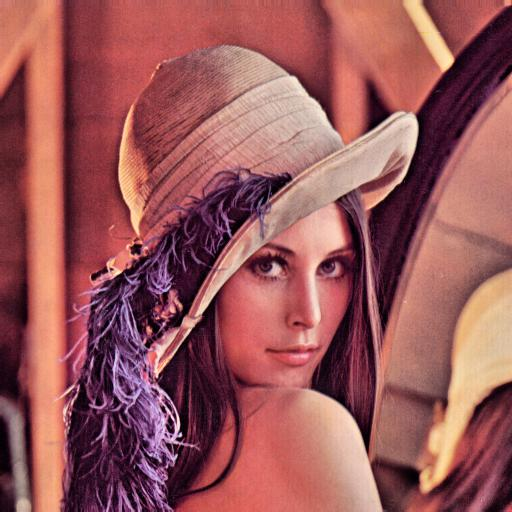
\includegraphics[width = 2.15in]{img/ConceptosTeoricos/LennaEqualized}}
\caption{Ecualización adaptativa}
\label{LennaEqua}
\end{figure}

\section{Reducción de ruido - Algoritmo Chambolle}
\label{ReduccionRuido}
El ruido de una imagen \cite{wiki:ImageNoise} consiste en variaciones en el color y brillo de los píxeles, de forma agresiva, al tomar imágenes mediante dispositivos de fotografía digital, como en nuestro caso, el microscopio electrónico. Reducir este ruido permite mejorar la visualización general de las imágenes y los objetos que contiene a cambio de disminuir el enfoque en la misma.

El algoritmo \textit{Chambolle} \cite{chambolle2004algorithm} es una técnica que, mediante la minimización del total de variación de una imagen \cite{wiki:TotalVariation}, consigue reducir el ruido sin que ello suponga un suavizado excesivo de los bordes en los objetos de la imagen, lo cual es interesante para este proyecto como vemos en la figura \ref{fig:chambolle}.

\begin{figure}[H]
\centering
\subfloat[Imagen original]{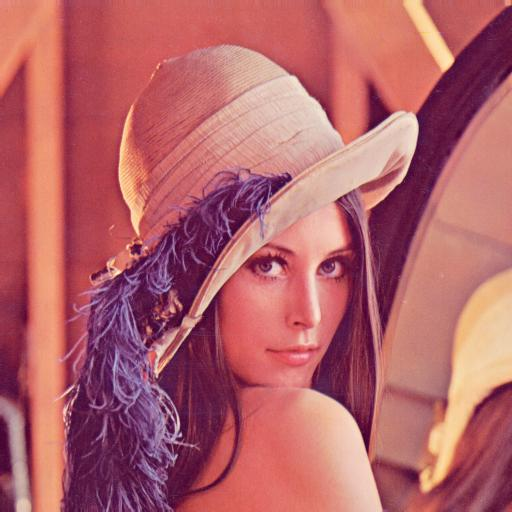
\includegraphics[width = 2.15in]{img/ConceptosTeoricos/LennaOriginal}}
\subfloat[Imagen suavizada]{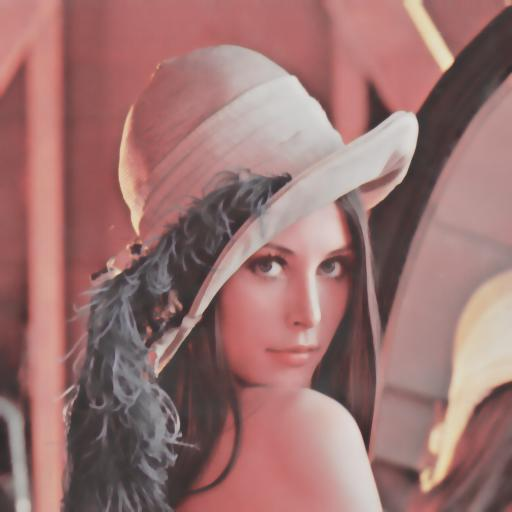
\includegraphics[width = 2.15in]{img/ConceptosTeoricos/LennaDenoise}}
\caption{Reducción de ruido \textit{Chambolle}}
\label{fig:chambolle}
\end{figure}

Parte de la premisa de que a una imagen se le ha aplicado un filtro y además se le ha añadido ruido gaussiano \cite{wiki:gaussianNoise} y trata de resolver un problema de ingeniería inversa para recuperar la imagen original \cite{articuloTotalVariation}.

\section{Aplicación de filtros}
Para poder aplicar un filtro a una imagen tendremos en cuenta los siguientes elementos:

\subsection{Kernel}
El kernel, también llamado máscara o matriz de convolución, consiste en una matriz cuadrada de dimensión normalmente impar\footnote{Encontramos excepciones como el operador de Robert con kernels de 2x2 \cite{wiki:RobertOperator}.} que, mediante la operación de convolución, aplicamos a una imagen para obtener la imagen filtrada. Existen filtros muy variados \cite{wiki:TiposFiltros}, algunos centrados en
desenfocar la imagen, añadirle contraste, eliminar ruido o realzar bordes para su detección como en nuestro caso.

Dependiendo del filtro que se quiera aplicar encontraremos unos kernels u otros como podemos ver en las figuras \ref{fig:KernelsPrewitt} y \ref{fig:KernelsSobel}. Un conjunto de kernels se suelen agrupar bajo el nombre de operador.

\begin{figure}[H]
    \centering
    \begin{bmatrix}
    1 & 0 & -1  \\
    1 & 0 & -1  \\
    1 & 0 & -1 
    \end{bmatrix}
    \begin{bmatrix*}
    1 & 1 & 1  \\
    0 & 0 & 0  \\
    -1 & -1 & -1 
    \end{bmatrix*}
    \caption[Kernels Prewitt]{Kernels Prewitt \cite{wiki:Prewitt}}
    \label{fig:KernelsPrewitt}
\end{figure}

\begin{figure}[H]
    \centering
    \begin{bmatrix*}
    -1 & 0 & 1  \\
    -2 & 0 & 2  \\
    -1 & 0 & 1 
    \end{bmatrix*}
    \begin{bmatrix*}[r]
    -1 & -2 & -1  \\
    0 & 0 & 0  \\
    1 & 2 & 1 
    \end{bmatrix*}
    \caption[Kernels Sobel]{Kernels Sobel \cite{wiki:Sobel}}
    \label{fig:KernelsSobel}
\end{figure}

Sus dimensiones son impares para poder identificar el elemento central de la matriz que se utilizará en la operación de convolución.

\subsection{Convolución} 
\label{ct:convolucion}
La operación de convolución nos permitirá conseguir una imagen filtrada, para ello necesitaremos un kernel y una imagen, considerándola como una matriz de dos dimensiones.

Citando el proyecto anterior \cite{perikymataV1}, la operación consiste en pasar por todos los puntos de la imagen, a los que se superpone el kernel, de modo que el elemento central coincida con el punto de la imagen en el que nos encontremos. Seguidamente se multiplican los valores del kernel por los valores de los puntos de la imagen sobre los que está superpuestos y se suman todos. El resultado será el nuevo valor que toma el píxel en el que nos encontramos como podemos ver en la figura \ref{fig:ProcesoConvolucion}.

\imagenCustomSinRef{img/ConceptosTeoricos/Convolucion}{Proceso de convolución \cite{perikymataV1}}{ProcesoConvolucion}{0.9}{Proceso de convolución}

\section{Filtros de detección de bordes}
Antes de comenzar con la explicación de los filtros, conviene repasar unos conceptos de interés sobre lo que veremos más adelante.

Los filtros de detección de bordes nos permiten conseguir que los valores máximos y mínimos de una imagen queden bien diferenciados. Estos filtros están basados en operadores derivativos ya que, al hacer la derivada a lo largo de la imagen, consiguen que la variación luminosa sea máxima y por tanto se marcan más los bordes \cite{ubu:ApuntesHardware}. En este proyecto encontraremos los siguientes tipos de filtros:
\begin{itemize}
    \item Filtros en la primera derivada:\label{ct:PrimeraDerivada}\\    
    Los operadores que calculan la primera derivada se llaman \textit{gradientes}. Algunos de estos operadores son: Sobel \cite{wiki:Sobel}, Prewitt \cite{wiki:Prewitt} y Robert \cite{wiki:RobertOperator}. Generalmente se computan en dos ejes, \textit{x} e \textit{y} para después sumarse y conseguir el gradiente completo junto con la imagen con bordes resaltados.
    \item Filtros en la segunda derivada: \label{ct:SegundaDerivada}\\   
   En la segunda derivada encontramos filtros como los laplacianos y otros como los hessianos. Los filtros laplacianos calculan la suma de la segunda derivada y dan como resultado un escalar\footnote{Número perteneciente a los reales.}, mientras que los filtros hessianos calculan una matriz con todas las posibles combinaciones de las segundas derivadas, la matriz hessiana \cite{wiki:HessianMatrix}.
   
   A diferencia de los operadores gradiente estos son todavía más sensibles al ruido de la imagen.
\end{itemize}

A continuación se mencionan los filtros de detección de bordes más relevantes con los que se ha trabajado y sus características:

\subsection{Kirsch}
\label{Kirsch}
El filtro de Kirsch es un operador de gradiente, por lo que al aplicarlo acentúa los bordes. Según se explica en \cite{scholar:venmathi2016kirsch}, como característica fundamental tendremos distintos \textit{kernels} en función de la orientación de los bordes que queremos resaltar, algunos como los de la figura \ref{fig:KernelsKirsch} para marcar bordes horizontales, verticales o ligeramente inclinados.

%Necesario importar un par de paquetes en el archivo de memoria principal
\begin{figure}[H]
    \centering
    \begin{bmatrix*}[r]
    +5 & +5 & +5  \\
    -3 & 0 & -3  \\
    -3 & -3 & -3 
    \end{bmatrix*}
    \begin{bmatrix*}[r]
    +5 & +5 & -3  \\
    +5 & 0 & -3  \\
    -3 & -3 & -3 
    \end{bmatrix*}
    \begin{bmatrix*}[r]
    +5 & -3 & -3  \\
    +5 & 0 & -3  \\
    +5 & -3 & -3 
    \end{bmatrix*}
    \caption[Kernels Kirsch: Norte, Noroeste y Oeste]{Kernels Kirsch: Norte, Noroeste y Oeste \cite{scholar:venmathi2016kirsch}}
    \label{fig:KernelsKirsch}
\end{figure}

Como se puede observar en la figura \ref{fig:KirschEffects}, el efecto conseguido guarda una relación contraria con el nombre del kernel, pues el filtro norte resalta los bordes horizontales y el filtro oeste resalta los verticales. 

El nombre de la orientación se refiere a los elementos del kernel que multiplicarán positivamente en la operación de convolución (sección \ref{ct:convolucion}), en este caso los elementos con valor \textit{+5}. Así, el kernel oeste se llama así por encontrar todos los \textit{+5} en dirección oeste.

\begin{figure}[H]
\centering
\subfloat[Imagen original]{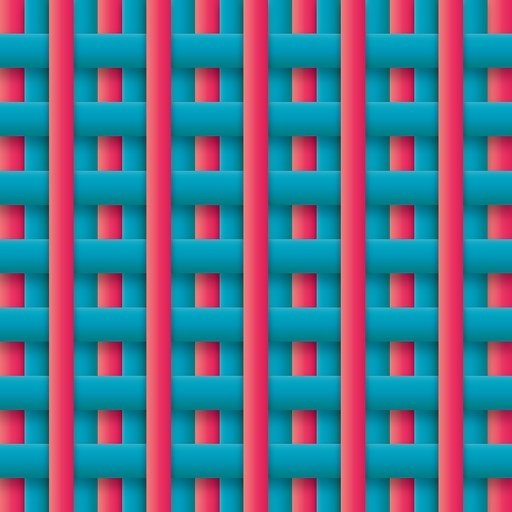
\includegraphics[width = 1.7in]{img/ConceptosTeoricos/Square}}
\subfloat[Kirsch Norte]{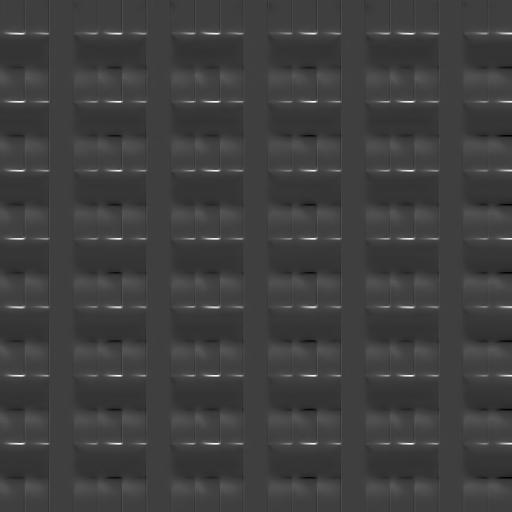
\includegraphics[width = 1.7in]{img/ConceptosTeoricos/SquareNorth}}
\subfloat[Kirsch Oeste]{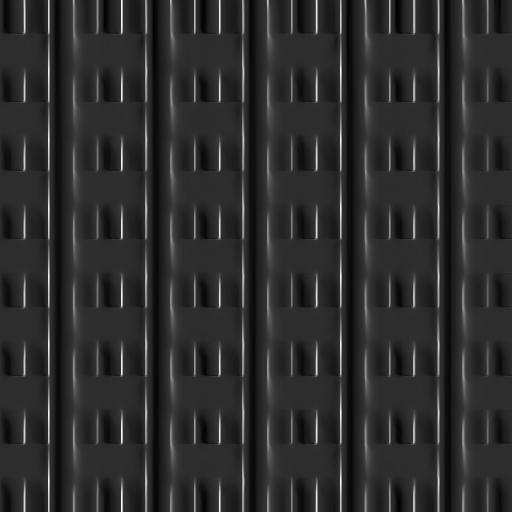
\includegraphics[width = 1.7in]{img/ConceptosTeoricos/SquareWest}}
\caption{Efectos del filtro Kirsch}
\label{fig:KirschEffects}
\end{figure}

\subsection{Frangi}
\label{Frangi}
Frangi \cite{skimage:Frangi} es una modificación del filtro hessiano (sección \ref{ct:SegundaDerivada}). Se utiliza en la detección de bordes continuos como por ejemplo ríos, arrugas o venas. Está basado en el cálculo de los máximos eigenvectores\footnote{Valores que no cambian cuando se aplica una modificación \cite{wiki:Eigenvector}.} sobre la matriz hessiana. Aplicado a la imagen de Lenna \cite{wiki:Lenna} quedaría como en la figura \ref{fig:FrangiFilter}.

\imagenCustom{img/ConceptosTeoricos/LennaFrangi}{Filtro Frangi}{FrangiFilter}{0.7} 

\section{Marcado de bordes}
En esta sección se comentarán los procesos que se llevan a cabo después de la aplicación de los filtros para realzar las perikymata.

\subsection{Binarización}
\label{Binarizacion}
El proceso de binarización (figura \ref{fig:Binarize}) consiste en conseguir que los valores de una imagen tomen solo dos posibles valores, generalmente un \textit{true} o \textit{false} lógicos, lo cual se traduce visualmente en una imagen en blanco y negro.

El procedimiento se basa en pasar por todos los puntos de una imagen, comparando su valor con un cierto valor \textit{umbral} y sustituir el valor del punto por un \textit{true} o \textit{false} (o también \textit{0} o \textit{1}) si es mayor o menor que el \textit{umbral}.

\begin{figure}[h]
\centering
\subfloat[Filtro Kirsch Oeste]{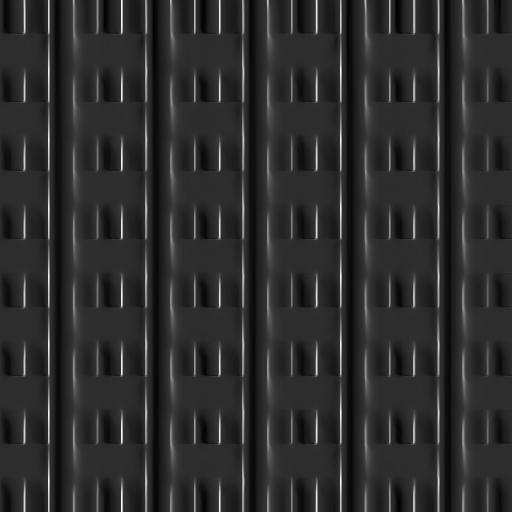
\includegraphics[width = 2.4in]{img/ConceptosTeoricos/SquareWest}}
\subfloat[Imagen binarizada]{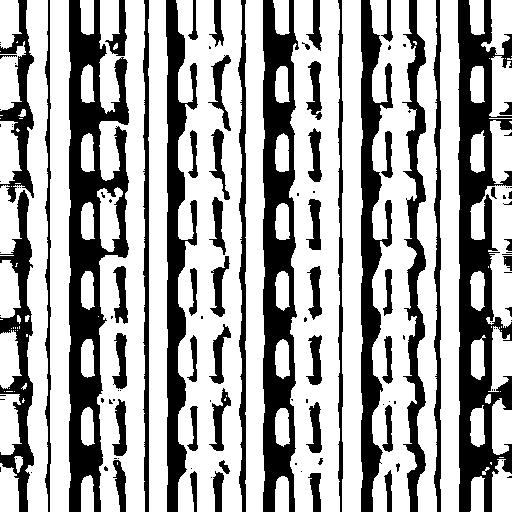
\includegraphics[width = 2.4in]{img/ConceptosTeoricos/SquareBinarize}}
\caption{Efectos de la binarización}
\label{fig:Binarize}
\end{figure}
\FloatBarrier

\subsection{Esqueletonización}
\label{Esqueletonizacion}
La esqueletonización es el procedimiento que aplicamos a una imagen binarizada para que su valor lógico \textit{true} se reduzca al tamaño de un píxel, normalmente dando lugar a líneas a lo largo de la imagen. Esto es útil, ya que si en la imagen los bordes están realzados, permitirá que queden muy marcados (como en la figura \ref{fig:Skeletonize}) y sea fácil su posterior identificación.

\begin{figure}[H]
\centering
\subfloat[Imagen binarizada]{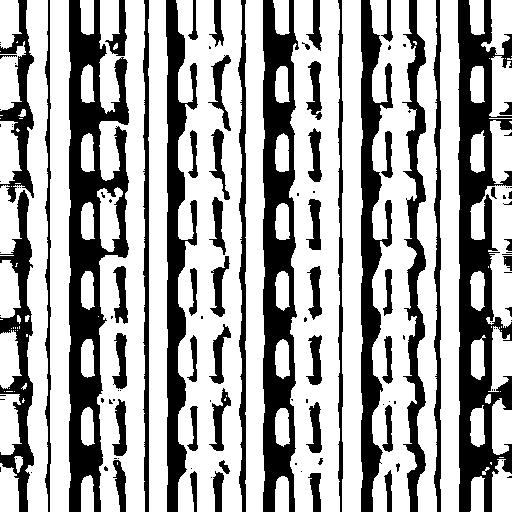
\includegraphics[width = 2.4in]{img/ConceptosTeoricos/SquareBinarize}}
\subfloat[Imagen esqueletonizada]{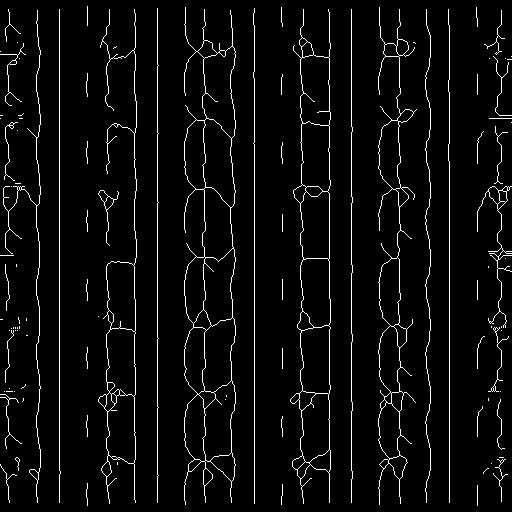
\includegraphics[width = 2.4in]{img/ConceptosTeoricos/SquareSkeletonize}}
\caption{Efectos de la esqueletonización}
\label{fig:Skeletonize}
\end{figure}


\section{Detección de líneas}
\label{Hough}
La detección de líneas se lleva a cabo mediante la Transformada de Hough.

La \textit{Transformada de Hough} es un mecanismo desarrollado para visión computacional, utilizado normalmente para la extracción de líneas e identificación de círculos y elipses en imágenes. Requiere que las imágenes estén binarizadas y con la menor cantidad de ruido posible.

Cuenta con múltiples variaciones, la función utilizada en el proyecto \cite{skimage:HoughLine} implementa la \textit{Transformada Probabilística de Hough Progresiva} desarrollada en este artículo \cite{galamhos1999progressiveHough} y, como característica diferenciadora de la \textit{Transformada Probabilística de Hough} tradicional, reduce el coste computacional y opera sobre los ángulos especificados como vemos en la figura \ref{fig:HoughDetected}. 

\imagenCustomSinRef{img/ConceptosTeoricos/SquareDetected}{Líneas detectadas sobre la figura \ref{fig:Binarize}b}{HoughDetected}{0.7}{Imagen con líneas detectadas}

Esta operación, en vez de desarrollarse sobre toda la imagen, se centra en áreas concretas que tienen mayor probabilidad de contener una líneas.

\newpage
\section{Espacios de color} \label{ct:EspaciosColor}
Una imagen es considerada una matriz de dos dimensiones, donde cada píxel guardar cierta información que podemos interpretar en distintos modelos de color. En este proyecto se manejan dos modelos de colores.

\subsection{Modelo RGB - RGBA}
El modelo \textit{RGB} \cite{wiki:RGB} interpreta el color gracias a la combinación de los tres colores primarios: rojo (R), verde (G) y azul (B). 

Los colores primarios toman valores enteros entre 0 y 255, siendo este último el valor de máxima intensidad. Este espacio de color es el utilizado en toma de imágenes digitales.

En determinados tipos de imágenes, como las imágenes \textit{png}, se añade además el canal \textit{alpha} (A), que indica la transparencia del color. Podemos encontrar variaciones en los rangos del canal \textit{alpha} dependiendo de la tecnología usada, por ejemplo, en hojas de estilo CSS el rango del canal es un número decimal entre \textit{0} y \textit{1} y en la lectura de imágenes con Python es un número entero entre \textit{0} y \textit{255}.

Al leer los datos de un píxel en Python, siguiendo este modelo, encontraríamos un vector como el de la figura \ref{fig:RojoRGB}.

\begin{figure}[H]
    \centering
    \begin{bmatrix*}[r]
        255 & 0 & 0 & 255 
    \end{bmatrix*}
    \caption{Color rojo en RGBA}
    \label{fig:RojoRGB}
\end{figure}

\subsection{Modelo HSV}
\label{ModeloHSV}
El modelo \textit{HSV}\footnote{También conocido como \textit{HSB} (\textit{Brightness}), guarda similitud con otros espacios de color como \textit{HSI} o \textit{HSL} aunque no llega a ser el mismo debido a la forma de conversión desde \textit{RGB} \cite{wiki:spaceHSV_HSI_HSL}.} \cite{wiki:spaceHSV_HSI_HSL} representa los colores dividiéndolos en:
\begin{itemize}
    \item \textit{Hue}: consiste en el matiz del color. Se mide en grados sexagesimales.
    \item \textit{Saturation}: se corresponde con la saturación del color e indica su intensidad. Generalmente se mide con porcentajes.
    \item \textit{Value}: indica el brillo del color. Al igual que con la saturación se mide en porcentajes.
\end{itemize}

\pagebreak
Este modelo es utilizado en selectores de colores debido a la sencillez de compresión para el ser humano. Podemos identificar los colores según el ángulo como en la figura \ref{fig:HSVCircle}.

\imagenCustomSinRef{img/ConceptosTeoricos/HSVcircle}{Rueda de matices HSV \cite{ForoOpenCV}}{HSVCircle}{0.5}{Matices HSV}

La utilidad para este proyecto radica en que se definirá un rango dentro del matiz para considerar qué es rojo y qué no y se identificarán como perikymata las líneas con colores en ese rango.

Consideraremos rojo todo color con un matiz entre 350º y 10º y con una saturación y brillo superiores al 80\%.


